\section{System Description}

The cloud is a service where all the application can be executed on a virtual 
environment owned either by private or company. In our application, we used the 
Internet of Things (IoT) Hub from Azure, which is a centralized platform that facilitates the 
connections and the management of fleets of IoT devices. The IoT Hub enables a streamlined 
bidirectional comunication from the Cloud to the physical devices, sensors.
As reported above, nowadays most of the energy plant are equipped with SCADA 
(Supervisory Control and Data Acquisition) \cite{daneels1999scada}, which enables data 
real-time monitoring and control of industrial processes and infrastructure.
It integrates hardware and 
software components to collect data from sensors, control equipment, and provide 
centralized oversight through Human-Machine Interfaces (HMIs). However, in comparison with SCADA, the IoT Hub has some more 7
support in terms of scalability, as it can support thousand of sensors and embedded devices, and also provide an extra layer of 
flexibility in terms of data collection for real-time and historical data. Moreover, it also provides different technologies for 
data driven modelling and artificial intelligence services. 

IoT sensors can be controlled singularly from the Azure Hub, but this is not our case. In our application, all the sensors are 
aggregated using a Kunbus Revolution Pi, which is the industrial standard of Revolution Pi. 
The Revolution Pi enables a bi-directional communication and serves as bridge between the PLC and the Cloud. 
The communication between the Gateway and the PLC is Modbus TCP/IP, a tailored version of the protocol for network communication 
over internet. One of the key advantage of this chain strategy is that the majority of the sensors, VDFs are connected to the 
PLC directly, so there is not need to rebuild from scratch the communication between all the sensor and the RevPi. 
The PLC is the Siemens s7-1200, which support Profinet, a propetary version of Profibus protocol, developed by Siemens that enable fast and reliable communication in control. 
The PLC is the connected to the following devices: VDF1, VDF2, VDF3, Outflow sensor, level sensor, pressure sensor, 
Addionally, from each VDF can be retrieved the instantaneous speed and power consumption. 

A crucial role in this application is played by the RevPi which not only combine the collected data from the 
PLC and the gateway and pushes the data to the cloud but also acts as real-time controller, overcoming the limitation 
of the PLC in terms of computational capabilities. In fact, the needs more comprehensive and optimization based control techniques 
, poses the needs of extra computational power, memory allocation and faster CPUs.
This architecture, compared to purely cloud-based controller, provides an extra layer of security, as the the on-site control device, can able to handle different 
situations, overcoming well-known limitations broader adoption, as delays or disruptions in communications.


\begin{figure}[h]
    \centering
    \hspace{2cm}
    \includegraphics[width=0.5\textwidth]{img/schematic.pdf}
    \caption{Your caption text.}
    \label{fig:your_label}
\end{figure}


\subsubsection{Data streaming and Features.}
The resolution frequency of the data streaming is $1\si{\hertz}$, as every second one measurement is sampled, pushed and stored to a time series database 
located in the cloud. Each sensor has a time index and values and can be queried from external APIs. 
This architecture allows high modularity as different blocks perform different operation



\begin{table}[!t]
    \renewcommand{\arraystretch}{1.3}
    \caption{Sensors Overview}
    \centering
    \label{table_1}
    \resizebox{0.8\columnwidth}{!}{
        \begin{tabular}{c c c}
            \hline\hline \\[-3mm]
            \multicolumn{1}{c}{Sensor} & \multicolumn{1}{c}{Unit of Measurement} & \multicolumn{1}{c}{Protocol} \\[1.6ex] \hline
            $ \rm{Level} $  & \si{\meter} & \textit{Analog} \\
            $ \rm{Speed} $ & \si{rpm} & \textit{Profinet} \\ 
            $ \rm{Inflow} $ & \si{\meter^3}/\si{\hour} & \textit{Virtual} \\ 
            $ \rm{Power} $ & \si{kW}/\si{\hour} & \textit{Profinet} \\ 

            $ \rm{Pressure} $  & \si{psi} & \textit{Profinet} \\
            $ \rm{Outflow} $ & \si{\meter^3}/\si{\hour} & \textit{Analog} \\ 

            \hline\hline
        \end{tabular}
    }
\end{table}


\begin{figure}[H]
    \centering
    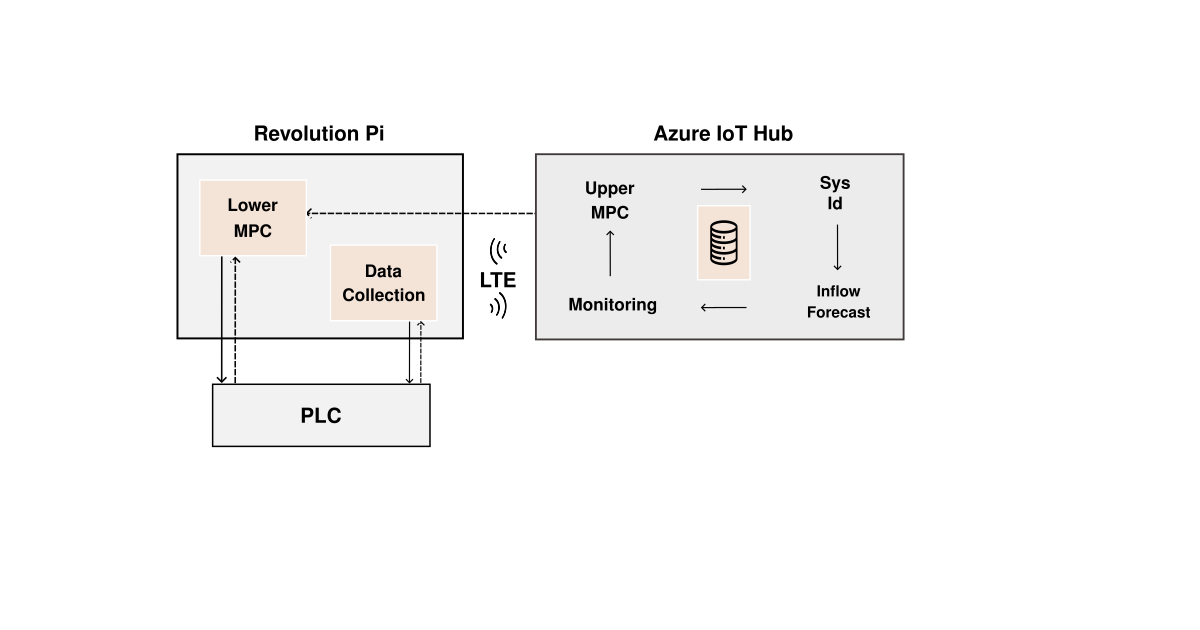
\includegraphics[width=0.49\textwidth]{img/block_diagram.pdf}
    \caption{Edge-Cloud Architecture }
    \label{fig:your_label}
\end{figure}